\documentclass[11pt]{beamer}
\usepackage[utf8]{inputenc}
\usepackage[spanish]{babel}
\usepackage{amsmath}
\usepackage{amsfonts}
\usepackage{amssymb}
\usepackage{graphicx}
\usepackage{lipsum}
\usepackage{ragged2e}
\usepackage{hyperref}
\usepackage{float}
\usepackage{url}
\usetheme{Madrid}
\usecolortheme{beaver}
\newcommand{\celda}[1]{
	\begin{minipage}{2.5cm}
		\vspace{5mm}
		#1
		\vspace{5mm}
	\end{minipage}
}

\author[Camila and Adriana]{Camila Andrea Suarez and Adriana Romero}
\title[Presentation paper]{The Long-Run Effects of the Scramble for Africa} 
\subtitle{Stelios Michalopoulos and Elias Papaioannou}
\institute[]{
	\inst{}
		Pontificia Universidad Javeriana\\
			\vspace{2mm}
	\inst{}
		Economic Growth and Comparative Development
}

\AtBeginSection[]
{
\begin{frame}<beamer>{Content}
\tableofcontents[currentsection,currentsubsection]
\end{frame}
}

\begin{document}

\begin{frame}
\maketitle
\end{frame}

\begin{frame}{Content}
\tableofcontents
\end{frame}
	
\section{Historical Background}
\begin{frame}{Historical Background}
\begin{itemize}
\item Scramble for Africa 
\pause
\item Europeans had limited knowledge of local conditions
\pause
\item The population belongs to ethnic groups that are partitioned among different states
\end{itemize}
\end{frame}

\begin{frame}{Aspects of the Scramble for Africa}
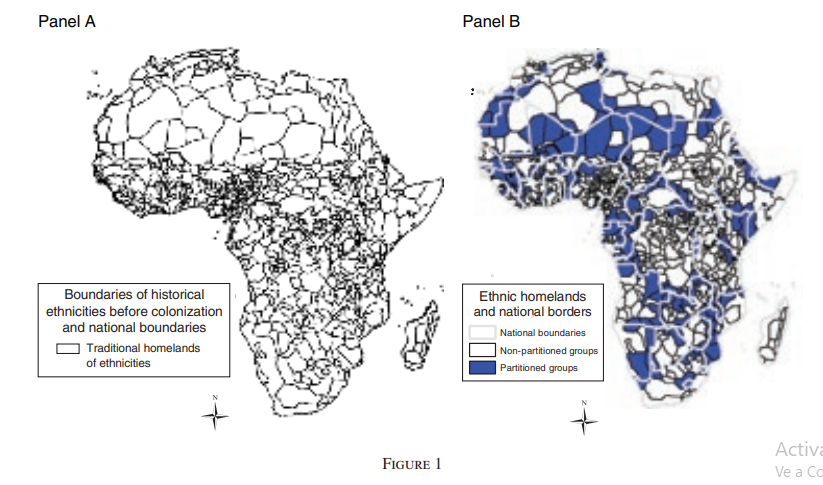
\includegraphics[width=12cm]{PresentacionPaper/map1.png}  
\centering
\end{frame}	

\section{Research objective}
\begin{frame}{Research objective}
\justifying Explore the consequences of ethnic partitioning for African groups, where the arbitrary design of the border and the large number of divided groups offer the opportunity to identify the impact of partitioning.
\end{frame}

\section{Literature}
\begin{frame}{Literature}
\justifying 
\begin{itemize}
\item Asiwaju 1985; Wesseling 1996; Dowden 2008; Thomson 2010) have maintained that the main channel of Europeans’ influence on development was not colonization per se, but the improper border design. 
\pause
\item Herbst (2000, p. 94) The boundaries were, in many ways, the most consequential part of the colonial state. The artificial
borders fostered ethnic struggles and conflict primarily by splitting groups across the newly-minted African states.
\pause
\item Alesina, Easterly, and Matuszeski (2011), Show that countries with more straight-line-like borders and nations where a significant part of their population also resides in different countries underperform economically.
\end{itemize}
\end{frame}

\section{Data}
\begin{frame}{Data}
\justifying
\begin{itemize}
\item Using a newly-assembled dataset, Armed Conflict Location and Event Data Project (ACLED)
\pause
\item Uppsala Conflict Data Program Georeferenced Event Dataset, UCDP-GED 
\pause
\item The Ethnic Power Relations (EPR) dataset (Wimmer, Cederman, and Min 2009)
\pause
\item Demographic and Health Surveys (DHS)
\end{itemize}
\end{frame}

\section{Data analysis}
\begin{frame}{TableA}
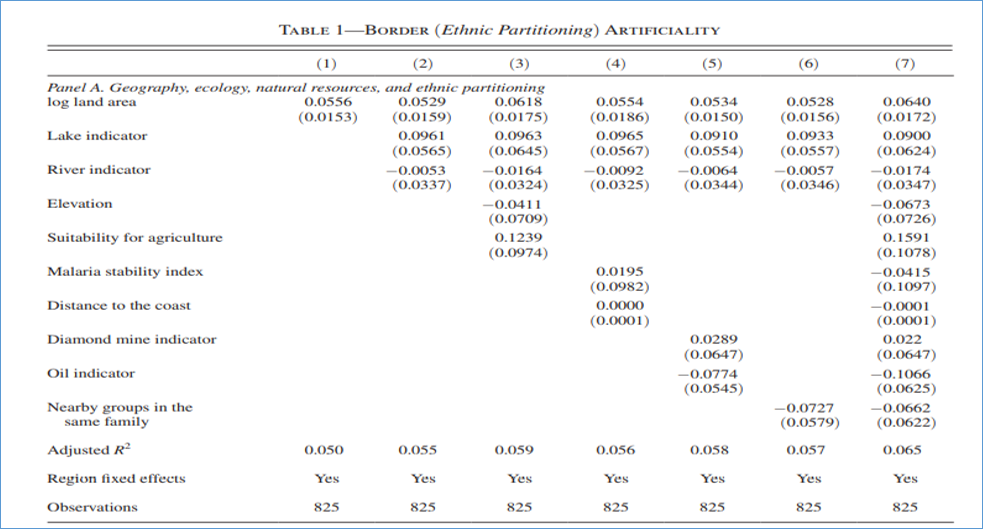
\includegraphics[width=12cm]{PresentacionPaper/Table1.png} 
\centering
\end{frame}

\begin{frame}{TableB}
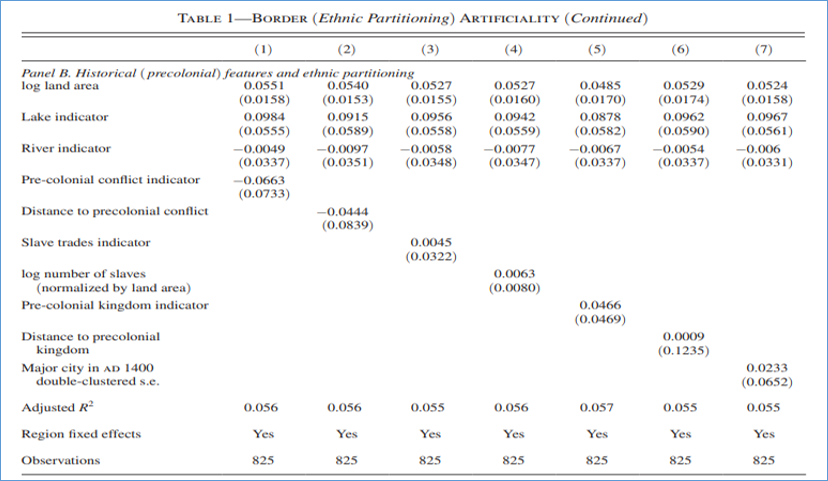
\includegraphics[width=12cm]{PresentacionPaper/Table1.1.png} 
\centering

\end{frame}	

\section{Econometric Specification and Estimation}
\begin{frame}{ Econometric Specification and Estimation}
\begin{align}
Y_{i,c} = \exp({a}_c+{\gamma}{SPLIT_{i,c}}+{\phi}{SPLI_{i,c}}+{X'_{i,c}}{\Phi}+\varepsilon_{i,c}),
\end{align}
\centering
\end{frame}

\begin{frame}{Table 2}
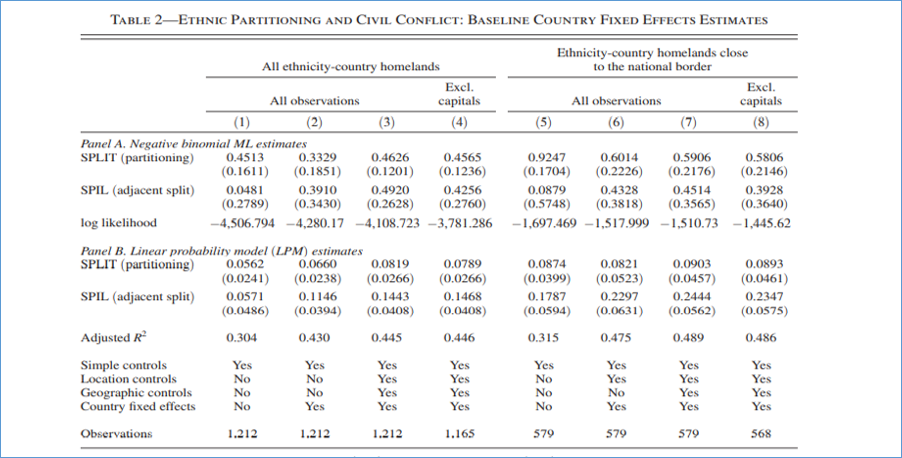
\includegraphics[width=12cm]{PresentacionPaper/Table2.png}
\centering
\end{frame}

\begin{frame}{Table 3}
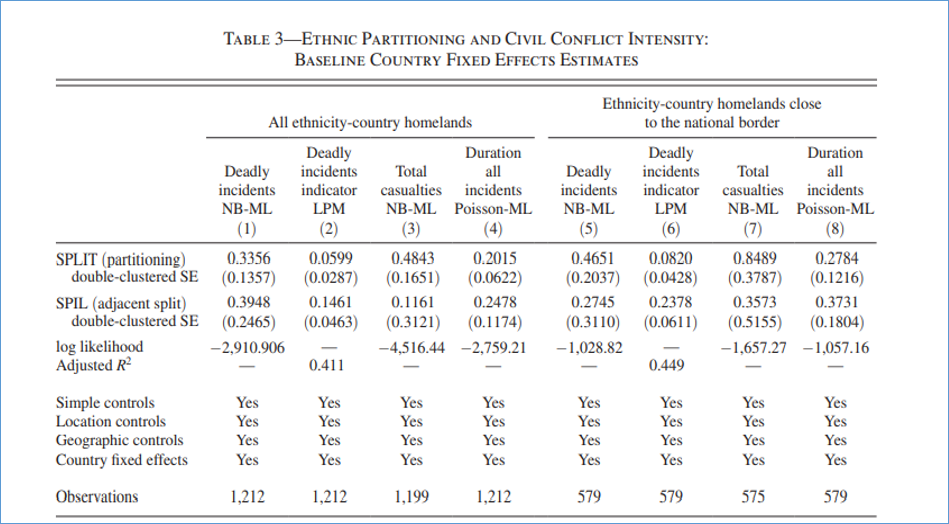
\includegraphics[width=12cm]{PresentacionPaper/Tabla3.png}   
\centering
\end{frame}

\begin{frame}{Table 4}
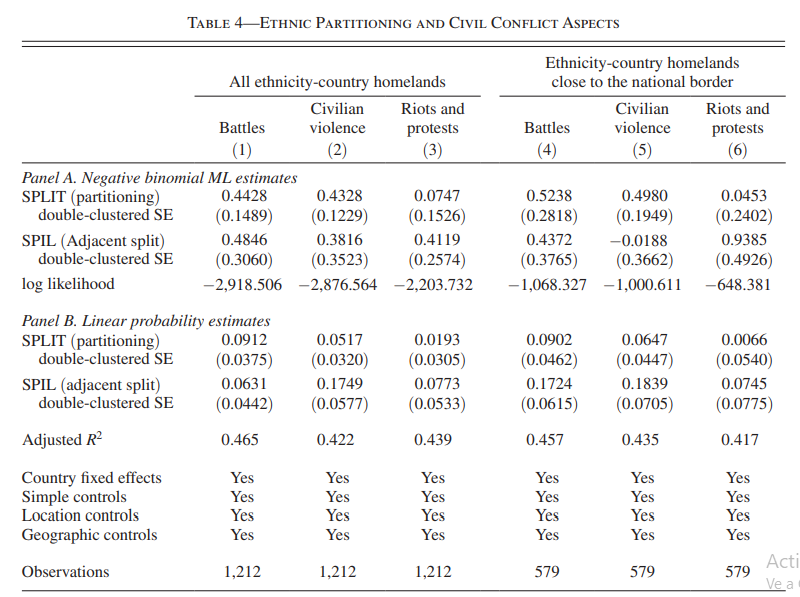
\includegraphics[width=10cm]{PresentacionPaper/Table4.png} 
\centering
\end{frame}

\begin{frame}{Table 8}
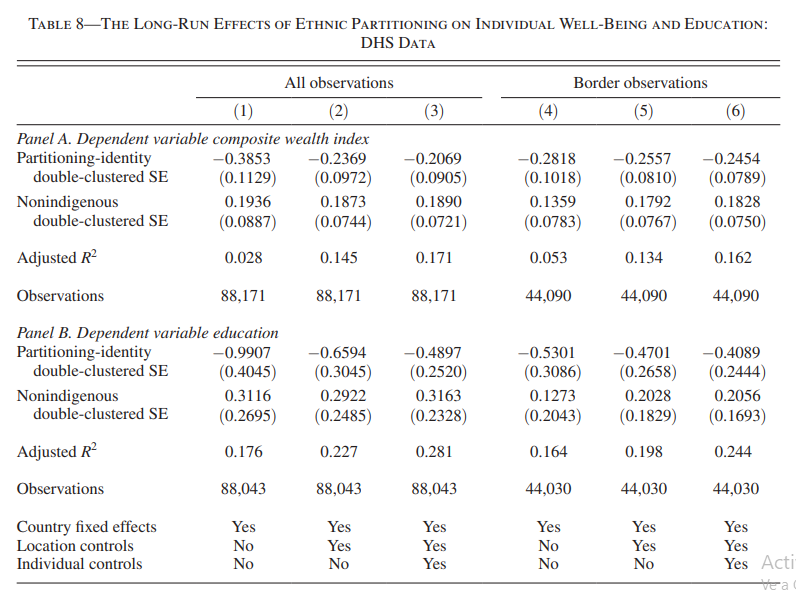
\includegraphics[width=10cm]{PresentacionPaper/Tabla8.png} 
\centering
\end{frame}

\section{Conclusion}	
\begin{frame}{Conclusion}
\justifying 
\begin{itemize}
\item There are no significant differences between divided and undivided lands taking into account various geographical and ecological features.
\pause
\item Estimates suggest that conflict intensity (likelihood) is approximately 40 percent (8 percent) higher in areas where partitioned ethnicities reside, as compared to homelands of ethnicities that have not been separated by national borders. 
\pause
\item The present evidence suggesting that neighboring countries use the homelands of partitioned groups to stage military interventions.

\end{itemize}
\end{frame}

\begin{frame}{Conclusion}
\justifying 
\begin{itemize}
\item Analysis shows that partitioned ethnicities are significantly more likely (11\%–14\% increased likelihood) to engage in civil wars that have an explicit ethnic dimension.
\pause
\item The likelihood that split ethnicities are subject to political discrimination from the national government is approximately 7 percentage points higher compared to non-split groups.
\pause
\item Members of partitioned groups have fewer household assets, poorer access to utilities, and worse
educational outcomes, as compared to individuals from non-split ethnicities in the same country.

\end{itemize}
\end{frame}

\end{document}
